
%!TeX spellcheck = en-US
%\chapter{Word Embedding and Distributional Features of the web-pages and texts}
\chapter{Open-set WGI with Neural Language Modeling}

\label{chap:word_embeddings}


%----------------------------------------------------------------------------------------

% Define some commands to keep the formatting separated from the content
\newcommand{\keyword}[1]{\textbf{#1}}
\newcommand{\tabhead}[1]{\textbf{#1}}
\newcommand{\code}[1]{\texttt{#1}}
\newcommand{\file}[1]{\texttt{\bfseries#1}}
\newcommand{\option}[1]{\texttt{\itshape#1}}

%----------------------------------------------------------------------------------------

\section{Introduction}\label{chap:word_embeddings:sec:intro}
 
\section{Neural Language Models}\label{chap:word_embeddings:sec:NLM}

\subsection{N-grams, Distributional Features and Word Embeddings} \label{chap:word_embeddings:sec:ngrans_vs_doc2vec}


The Bag of Terms (BOT) n-grams, a.k.a the Bag of Words (BOW), is the most common text modeling in NLP and other text related research domains. The assumption as in other features from other domain, say image processing, is the \textit{Independent and Identical Distribution (i.i.d)} of the terms, then it is easy to express context of a text into a \textit{fixed vector} sample which is the main requirement of most ML algorithms to work. Moreover, is computationally very easy and in the past the creation of such a fast document representing in respect of time consumption was critical due to the lack of the today's resources.

The BOT is still a top performance document representation however it comes to a great cost because it is loosing the order of the words and cannot capture their semantics. Therefore, it is impossible to capture similarities in word level such as "power" and "strength", in sentence level such as "Beats me!" and "I don't know", and in writing style such as "My greetings to..." and "Say hello to... for me". 

\textit{Word Embeddings} and \textit{Distributional Feature (DF)}s is the state-of-the-art in language modeling as a result in the advances of the \textit{Statistical Language Modeling} and particularly the \textit{Neural Probabilistic Language} modeling. Ultimately, the \textit{Paragraph Vector Continues Bag of Words (PV-BOW)} DF modeling can be used for complicated classification tasks such as WGI, where the BOT together with its complicated heuristics for additional feature extraction can only perform as good when the task is more tight the corpus. Although, as it will be explained later the DF models and word embeddings is a computationally expensive process is might be comparable to a sequential set of heuristics for extracting a variety of features in the effort of capturing the information missing from the BOT in the first place.  

In this section it is described the PV-BOW modeling in detail, which have been used in combination with the NNDR (the open-set Nearest Neighbours) on the WGI task with promising results. First, it is described the \textit{Neural Language Modeling (NLE)} concept and on the top of it the \textit{Continues Bag of Words  (CBOW)} and  \textit{Skip-Gram (SG)} modeling, which they are special modified \textit{Feedforward} and \textit{Recurrent Neural Network models respectively}.

The goal of \textit{Statistical Language Modeling (SLM) } is to learn \textit{joint probability distribution function} of word sequences, i.e. word n-grams. The main difference to the BOW and particularly to the word n-grams TF (or TF-IDF) model, is the \textit{semantic proximity} of the word's neighbouring in the sentences. Implicitly the WNG-TF models is also capturing some of this information and definitely not explicitly. Additionally, the SLM can always return an estimate value for n-grams never seen before, while for the WNG-TF this is impossible  \parencite{bengio2003neural}

The SLM model is defined as the \textit{joint conditional probability distribution} of the next word given the probabilities of previous ones as shown in equation \ref{chap:word_embeddings:eq:slm}

\begin{equation} \label{chap:word_embeddings:eq:slm}
	P(w = i) = \prod_{i=1}^{|V|} P(w_{i}|w_{i-k}, ... , w_{i+k})
\end{equation}
\noindent
where $w_{i}$ is the i-th word, and $k$ is for the number of words before or/and and after, writing sub-sequence $w_{i} = (w_{i-k}, w_{i-1}, ... ,w_{i+1}, w_{i+k})$. Note that this model returns a singleton value for a word on the condition of previews or/and next word. This model also can be expanded to have few more words in the conditional probability, usually from 2 up to 4. 

With this model it can be captured the semantic proximity but it will return zero in the case a sequence have never been met before in the samples. A solution to this problem is the interpolation or smoothness factor that can be applied such as in the \textit{back-off tri-gram model} (Katz, 1980 see in bengio2003neural). 

The model of equation \ref{chap:word_embeddings:eq:slm} can capture the joint probability of word-sequences in terms of feature vectors, however, it cannot capture the correlation of the words in terms of semantics. Models like LSI or LDA are methodologies also been tested in IR and NLP for capturing the semantics in the context of the n-gram based SLM. 

The goal of the DF models is to learn simultaneously the \textit{word feature vectors}, a.k.a \textit{Word Embeddings}, and the probability function or word sequences, a.k.a \textit{Distributional Features}. The word embeddings is a \textit{continuous vector space} where the words are positioned in \textit{Vocabulary} context, where the similarity of words can be learned. The word sequences are capturing the proximity of words in the paragraph (or sentence) context.

The DF models then are able to learning the \textit{Continuous Distribution of Words in Sequences} and not only their role in sentences (such as in eq.  \ref{chap:word_embeddings:eq:slm} model) or only their similarity (such as the LSI models). The DF modeling is a NLM procedure where Neural Networks are used for approximating the\textit{ joint probability distribution function of the continuous distributed feature-sequences}, where the probability features are associated to the words of the Vocabulary.

In practice the distributed features is the mapping of the Vocabulary words $V = \{w_{i}, i \in [1, |V|] \}$ to a real vector $\vec{t}(i) \in \mathbb{R}^{m}$. Then the semantic distance can be approximated by a NNet algorithm given the distribution of the words. The words are initially are having a vector 1-of-V representation, a.k.a. \textit{One-hot representation}. Then the probability of the a word $w_{i}$ in equation \ref{chap:word_embeddings:eq:slm} can be replaced by the real continues vector $t{i}$ and the conditional probability $P(.|.)$ to be approximated my a NNet function $\hat{p}(.)$. The $\hat{}$ (hat) is for symbolizing a special condition where the probability is approximated given a sequence with a specific order, say preceding words or succeeding words or both. 

Now the DF neural model can be calculated with several architectures where the $\vec{t}$ and the $\hat{p}$ continues distribution can feed separate layers of joint layers, and also the learning strategy can have variant implementations such as Continues Bag-of-Words, Skip-grams etc. The strategy of learning and the NNet architecture are very close related and the results are \textit{continues probability functions with substantially different meaning}, where they can either encode word similarities, word semantics or even paragraph and documents encoding and similarities. 

To begin with, the most general architecture is to use the \textit{Feedforward Neural Network} with a projection layer, a hidden layer and an output layer as shown in figure \ref{chap:word_embeddingss:fig:CBOW_diagram}. This NNet has an input layer where every word in the vocabulary is assigned to an One-hot vector $\hat{t}_{i}$ and all the sequence of the \textit{word vectors} are concatenated and forming the input vector $\hat{w}_{i}$ . The $\hat{w}$ is the input the projection layer $\vec{t} = \hat{w}W_{in}$ as show in the figure. The $W_{in}$ is the weight matrix of the projection layer with same regularization parameters $\theta$.

\begin{figure}[t]
	\begin{center}
    	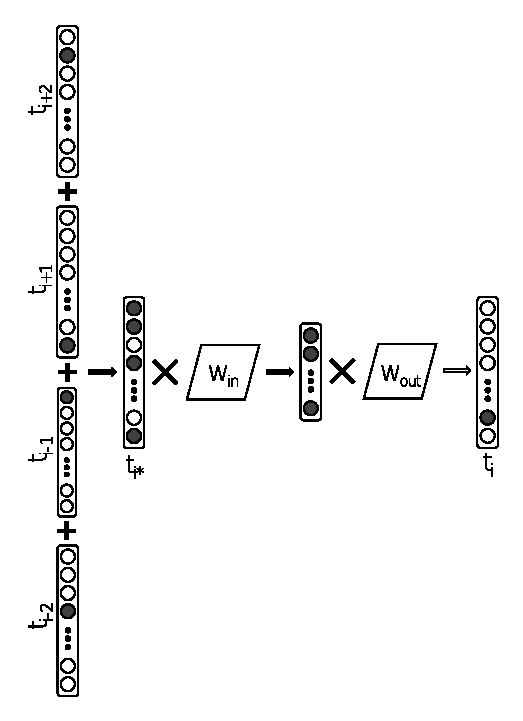
\includegraphics[scale=0.99]{Figures/CBOW_diagram.eps}
		\caption{Diagram for C-BOW and General NLM architecture. Depending whether the $t_{i*}$ is part of the projection and the hidden layer or the layers are different. In practice the weighting matrices are either shared or diff rent between the word projection and the hidden layer or it is the same matrix, which is equivalent to the words been projected to the same position as their vectors are averaged and not concatenated.}
		\label{chap:word_embeddingss:fig:CBOW_diagram}
	\end{center}
\end{figure}

Now the $\vec{t}$ is the input to a hidden layer $\vec{h}=\vec{t}H$, which is usually the \textit{hyperbolic tangent hidden layer}, where $H$ is the weights of the hidden layer. Then, the output $\hat{p}=\vec{h}W_{out}$ is the last layer of the NNet.

The generic architecture of the final output of the NLM described above is the equation \ref{chap:word_embeddingss:nlm_generic}. Note that the output vector $\vec{y}$ has size $|V|$ due to the input $\hat{w}$ and is the inference model of a \textit{continues distribution} of both the proximity of the words in the sentences (captured by the hidden layer) and the distribution over the vocabulary, which is the continues similarity of the words in this vocabulary. The output layer then is as described in equation \ref{chap:word_embeddings:eq:NLM}

\begin{equation} \label{chap:word_embeddings:eq:NLM}
	\vec{y} = \vec{t} + W_{out}(\vec{t}H + b_{h}) + b_{o}
\end{equation}

\noindent
where $b_{o}$ and $b_{h}$ are the output and hidden layers biases. Usually the Hidden layer typically has a size of 500 to 1000 neurons while the projection layer might be 500 to 2000. Due to the multiple layers and the feeding of both the projection and the hidden to the output layer there is great complexity and the process is very computationally demanding. 

A more efficient method is suggested in \parencite{mikolov2013efficient} where the non-linear hidden layer is removed and the projection layer is shared to all words, geometrically this is equivalent to the projection of the words to the same position. Then the algorithm is reformed and the $\hat{w}$ vectors are replaced by the $t^{*}$ which is the sum of the \textit{one-hot word vectors} \parencite{mitra2018introduction}. 

Now the equation \ref{chap:word_embeddings:eq:NLM} is becoming \ref{chap:word_embeddings:eq:CBOW}. Due to the new form of the NNet where the tangent hidden layer is absent, there is no constraint in the presenting sequence of the words order. Moreover, the succeeding words also can also be taken in to account in a given \textit{window} say for $k_{w}$ number of words around the specific one. 

\begin{equation} \label{chap:word_embeddings:eq:CBOW}
	\vec{y} = W_{out}(t^{*}W_{in}) + b_{o}
\end{equation}
The suggested algorithm is called \textit{Continues Bag-of-Words (CBOW)} because the words of the surrounding sequences is not important but it is still are taken into account for predicting the next word. Moreover the $\vec{y}$ has a size equivalent to the size of the Vocabulary $V$. 

In respect of training the CBOW model, a \textit{multiclass classifier} is set by a \textit{Softmax function} is described in equation \ref{} where the $y$ is the output of the equation \ref{chap:word_embeddings:eq:CBOW}. Note now the $\hat{p}$ continues probability is replaced by the $p$ district probability and because now the order in the words sequences are not important. Additionally, the $\vec{t}$ are replaced by the $t$ because it denotes that the words can be any term; character, words, word n-grams, character n-grams. 

\begin{equation} \label{chap:word_embeddings:eq:CBOW_softmax}
	p(t_{i}|t_{i-k},...,t_{i+k}) = \frac{e^{y_{t_{i}}}}{\sum^{|V|}_{i}{e^{y_i}}}
\end{equation}

The objective of the training of the NLM CBOW model is to maximize the conditional log probability in equation \ref{chap:word_embeddings:eq:CBOW_log_likelihood}. 

\begin{equation} \label{chap:word_embeddings:eq:CBOW_log_likelihood}
	 \mathcal{L}_{CBOW} = \frac{1}{|S|} \sum_{i=1}^{|S|}{\log{p(t_{i}|t_{i-k}, ... ,t_{i+k};\theta)}}
\end{equation}


\noindent
where $S$ is the \textit{set $k$-size of sampling windows} and  $\theta=\{b_{o},W_{in},W_{out}\}$ are the parameters and weights should be optimized in order the CBOW model to converge. \textit{Stochastic Gradient Decent} and \textit{Backpropagation} is used for training the NNet.

An other training strategy is the \textit{Skip-Gram} modeling, where the objective is to maximizes the log-likelihood of the equation \ref{chap:word_embeddings:eq:skipgram_log_likelihood}.

\begin{equation} \label{chap:word_embeddings:eq:skipgram_log_likelihood}
	 \mathcal{L}_{SkipGram} = \frac{1}{|S|} \sum_{i=1}^{|S|}{ \sum_{-k \leq j \leq +k}{ \log {p(t_{i+j}|t_{i};\theta)}  } }
\end{equation}
\noindent
where $S$ is the prediction windows over the training text and $k$ is the number of the words to be predicted surrounding the input word $\theta$ set of parameters to be optimized. The Softmax function of equation \ref{chap:word_embeddings:eq:skipgram_softmax} is applied at the output layer.

\begin{equation} \label{chap:word_embeddings:eq:skipgram_softmax}
	p(t_{i+k}|t_{i}) = \frac{ e^{(W_{out}  \times  t_{i+j})^{T} (W_{in} \times  t_{i})}}{\sum^{|V|}_{i}{ e^{(W_{out}  \times  t_{k})^{T} (W_{in} \times  t_{i})}}} 
\end{equation}
As shown in figure \ref{chap:word_embeddingss:fig:skipgram_diagram} the input and the output are one-hot vectors.

\begin{figure}[t]
	\begin{center} 
    	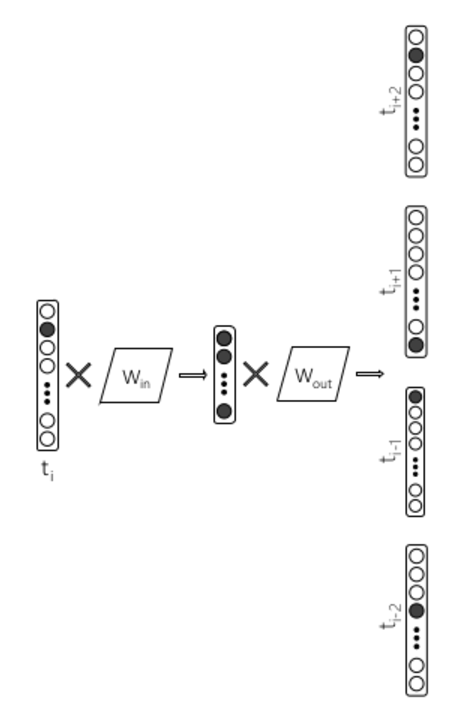
\includegraphics[scale=0.99]{Figures/skip_gram.eps}
		\caption{Diagram for Skip-Gram.}
		\label{chap:word_embeddingss:fig:skipgram_diagram}
	\end{center}
\end{figure}


Note that the two different weight matrices $W_{in}$ and $W_{out}$ (similarly to the CBOW) constitutes the $\theta$ set of parameters to be optimized of the models. $W_{in}$ gives the "in" embeddings corresponding to the input terms and $W_{out}$ corresponds to the output embeddings for the output terms. $W_{in}$, a.k.a. \textit{Word Embedding}, are used for several IR and NLP classification and regression tasks. The $W_{out}$ are usually discarded. 

A very important difference between the CBPW and Skip-Grams is the NNet architecture usually their implementation is based. Particularly, there are some internal detail occurring because of the objective ot the task. \parencite{boden2002guide}

Finally, all the above neural models, either CBOW or Skip-Grams, since they are approximating the continues distribution probability function of words over the the Vocabulary $V$ they have the constraint described in equation \ref{chap:words_embedding:eq:nnet_constraint}

\begin{equation} \label{chap:word_embeddings:eq:nnet_condtraint}
	\sum_{i=1}^{|V|}{p(t_{i}|t_{i-k}, ... ,t_{i+k})} = 1
\end{equation}

To summarize, the NLM models such as the CBOW are very effective \textit{Language Modeling} and it has the agility to measure simultaneously several properties form the context. That is, the distribution of the terms in the paragraphs of the texts and in the vocabulary and they are also called \textit{Distributional Features}. The features are set in a continues vector space and the model can return a prediction value $y$ (see equation \ref{chap:word_embeddings:eq:CBOW}) for set of terms given as an input at the test phase of the model and they can be treated as response signals of a text. Particularly a sequence of words.

The texts also now are considered as signal and the sequence of words now has a temporal property where the proximity and the order are providing important information. In respect of the term frequencies are still considered due to the temporal properties, where now the words with the higher TF are weighting or amplifying the sequential signal input to the network.

Finally, the training of the CBOW and the Skip-gram NLM is very expensive and although they have lower complexity than the more generic Feedforward Neural Networks with the tangent hidden layer explained above. However, there are several engineering solution that are accelerating the training even more such as the \textit{Huffman Binary Tree encoding or the Words} and \textit{Hierarchical soft-max}. The later is a solution where it is enabling us to use multi-processing and the $\theta$ parameters to be updated concurrently. The parallel asynchronous updating of the parameter matrices is not conforming to the mathematical constraints however in practice the negative effect is minor. 

The\textit{ Huffman Binary Tree} is a a methods for compressing the encoding of the terms where the one with the higher frequency to be accessed faster. In addition to this, \textit{negative sampling}, {sub-sampling}, or \textit{ramdom sampling} is also used where in the range of $k$ window for surrounding words only a few are selected during training with minor effect in  performance and significant acceleration in training. 

There are several detailed studies for \textit{Neural Language Modeling (NLM)}, Distributional Features and Word Embedding in \parencite{mitra2018introduction,mikolov2013efficient,mikolov2013distributed}. In the next paragraphs is explained thea \textit{Document to Vector (Doc2Vec)} Neural Model, where it is the extension of the above models CBOW and Skip-grams. Particularly, the PV-BOW is explained which has been used in this study on WGI, where a model of  the \textit{Continues Distribution of  Paragraphs} over the corpus context. Then, the web-pages are encoded in this continues distribution and their similarity is measured for the open-set WGI.
 
 
\subsection{Paragraph-Vector Bag-of-Words and Document Vectors Projection} \label{chap:word_embeddings:sec:PVBOW} 
 
In this study, the Paragraph Vector Bag-of-Words (PV-BOW) model is used for the WGI task in the open-set framework evaluation. The PV-BOW is a DF modeling of the documents as an extension of the Skip-Grams modeling. The PV-BOW extends the idea of the \textit{Continues Distribution of the Words} over the Vocabulary and the Context defined by a Corpus of documents. A \textit{Continues Distribution of the Paragraphs (CDP} is defined where this method considers the concatenation of the paragraph vector with the word vectors to predict the next word in a text window. 
 
The CDP can be derived with two methods, one is based on CBOW and the other on Skip-Grams, which is used in this study. The CBOW extension is called Distributed Memory Paragraph Vector (PV-DM) because the Paragraph Vector is given as an input together with the word vectors, and it is considered as memory of the words distribution.
 
Another way is to ignore the context words in the input, and make a model for predicting words randomly sampled from the paragraph in the output. That is the Skip-gram model but instead of a words the whole paragraph vector is given as an input as shown in figure \ref{chap:word_embeddingss:fig:PVBOW_diagram}. In practice, at each iteration of stochastic gradient descent, text window of $k$ size is sampled. Then a random word sampled from the text window and form a classification task given the Paragraph Vector and  this is the PV-DBOW. This model requires to store less data, because only the softmax weights are stored as opposed to both softmax weights and word vectors in the PV-DM. 

\begin{figure}[t]
	\begin{center} 
      	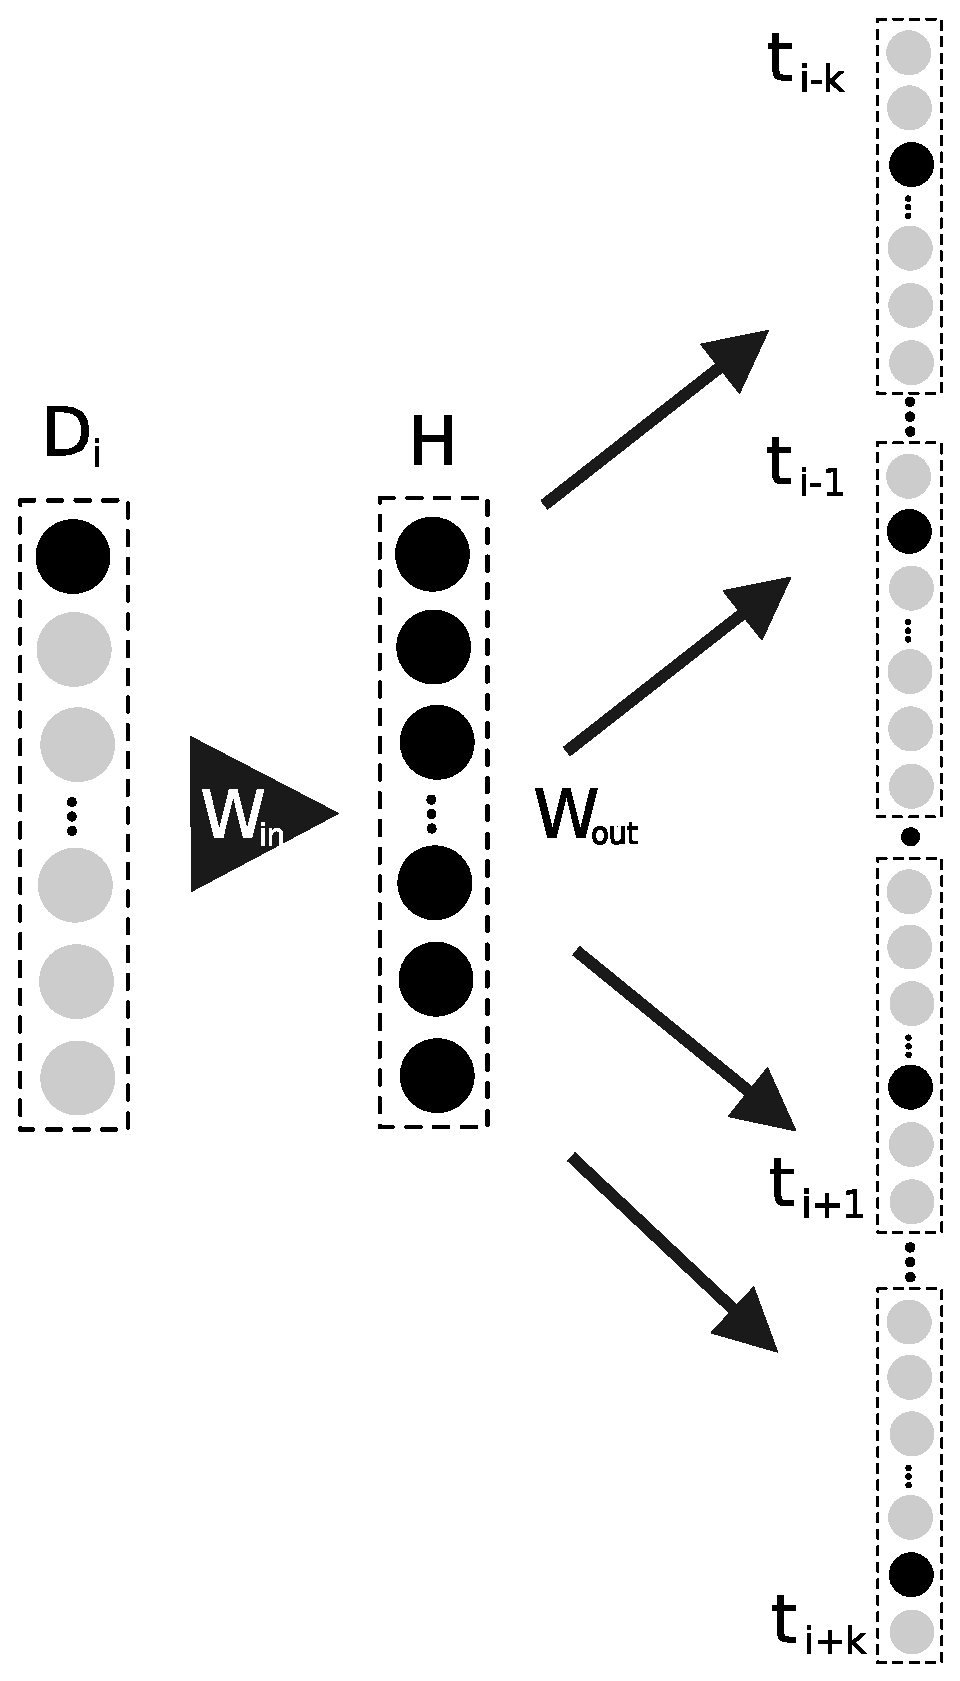
\includegraphics[scale=0.50]{Figures/pvbow.eps}
    		\caption{Diagram for PV-BOW}
		\label{chap:word_embeddingss:fig:PVBOW_diagram}
	\end{center}
\end{figure}


It should be noted that the Paragraph Vectors can be a text paragraph, a sentence, or the whole document. In this study, the whole web-pages is considered as shown in the first vector at the left in figure \ref{chap:word_embeddingss:fig:PVBOW_diagram}. There are several implementation for the PV-BOW modeling and a late evolution proposal for making the model more appreciate for IR problems. Including, \textit{Document frequency based Negative Sampling} and \textit{Document Length Regularization} \parencite{le2014distributed,posadas2017application}.

The PV-BOW objective log likelihood of Skip-gram models described in equation \ref{chap:word_embeddings:eq:skipgram_log_likelihood} is changing to the equation \ref{chap:word_embeddings:eq:pvbow_log_likelihood}  

\begin{equation} \label{chap:word_embeddings:eq:pvbow_log_likelihood}
	 \mathcal{L}_{SkipGram} = \frac{1}{|S|} \sum_{i=1}^{|S|}{ \sum_{-k \leq j \leq +k}{ \log {p(t_{i+j}|D_{i};\theta)}  } }
\end{equation}
\noindent
where $D_{i}$ is the Document Vector or Document ID, $S$ is the prediction windows over the training text and $k$ is the number of the words to be predicted surrounding the input word $\theta$ set of parameters to be optimized. Consequently,  the Softmax function is becoming as shown in equation \ref{chap:word_embeddings:eq:pvbow_softmax}.

\begin{equation} \label{chap:word_embeddings:eq:pvbow_softmax}
	p(t_{i+k}|t_{i}) = \frac{ e^{(W_{out}  \times  t_{i+j})^{T} (W_{in} \times  D_{i})}}{\sum^{|V|}_{i}{ e^{(W_{out}  \times  t_{k})^{T} (W_{in} \times  D_{i})}}} 
\end{equation}
Paragraph Vectors address some of the key weaknesses of bag-of-words (remember words can be any terms characters, words or POS) models. First, they capture the semantics of the terms. Therefore, words like “strong”  and "powerful" are closer together both and far from "Athens". Secondly, paragraph vectors take into consideration the word order, at least in sentence or paragraph level, in the same way that an Word n-Gram model would do in the size of n-Terms. As we will see experimentally the n-gram model also preserves a lot of information of the paragraph such as the word order. However, even if in some cases like in the experiments below, the n-grams perform equally to the PV-BOW DF models, the DF models can generalize better. They encoding more information with much denser and continuous dimemntionality or at least the information they capture is not sparse and maybe "broken" in the small ranges of n-terms.

In practice a library for HTML reprocessing and and Vector Representation of the web-pages has been created for this work, named  \textit{Html2Vec}\footnote{\url{https://github.com/dpritsos/html2vec}}. There as special module for PV-BOW modeling has been build, where it is based on the the algorithm can be found at \textit{Gensim package} \footnote{\url{https://github.com/RaRe-Technologies/gensim}}. 


In this study a PVBOW Distributional Feature model for the whole corpus is trained. The corpus initially is split to a set of paragraphs, as required from PVBOW. To be more specific the paragraphs are sentences split from all the document of the whole corpus. Then several models PVBOW feature models are trained for a variety of parameters and vector dimensions, explained in the experiments section below. After the model has been fitted then one vector for each web-document was inferred from the PVBOW. The final document vectors derived from \tetxit{Distributional Feature Model} are given to the open-set learning model explained below. 


\section{Experiments}\label{chap:word_embeddings:sec:experiments_setup}

\subsection{Corpus}\label{chap:word_embeddings:sec:experiments_corpora}

The experiments of this chapter, are based on \textit{SANTINIS}, a benchmark corpus already used in previous work in WGI \parencite{mehler2010genres_on_web,pritsos2018open,santini2007automatic}. Briefly, this dataset comprises 1,400 English web-pages evenly distributed into seven genres (blog, eshop, FAQ, frontpage, listing, personal home page, search page) as well as 80 BBC web-pages evenly categorized into four additional genres (DIY mini-guide, editorial, features, short-bio). In addition, the dataset comprises a random selection of 1,000 English web-pages taken from the SPIRIT corpus \parencite{joho2004spirit}. The latter can be viewed as \emph{unstructured noise} since genre labels are missing. More details for SATNINIS corpus are discussed in section \ref{}. 


\subsection{Open-set Models Parameters Setup}\label{chap:word_embeddings:sec:experiments_params}

To represent web-pages again the features are exclusively related to textual information, excluding any structural information, URLs, etc. The following representation schemes are examined: Character 4-grams (C4G), Word unigrams (W1G), and Word 3-grams (W3G). For each of these schemes, we use either Term-Frequency (TF) weights or DF features. The feature space for TF is defined by a vocabulary $V_{TF}$, which is extracted based on the most frequent terms of the training set --- we consider $V_{TF}=\{5k,10k,50k,100k\}$. The DF space is pre-defined in the PV-BOW model --- we consider $DF_{dim}=\{50,100,250,500,1000\}$.

In PV-BOW, the terms with very low-frequency in the training set are discarded. In this study, we examine $TF_{min}=\{3,10\}$ as cutoff frequency threshold. The text window size is selected from $W_{size}=\{3,8,20\}$. The remaining parameters of PV-BOW are set as follows: $\alpha=0.025$, $epochs=\{1, 3, 10\}$ and $decay=\{0.002, 0.02\}$. The PV-BOW creation process is also driven by an internal terms \textit{vocabulary} which is used for eliminating the terms with lower than a preferred frequency and then discards the terms from the text window for the PV-BOW (see section \ref{}).


Regarding the NNRD open-set classifier, there are two parameters, $lambda$ and DRT, and their considered values are: $\lambda =\{0.2, 0.5, 0.7\}$, $DRT\textit{=\{0.4, 0.6, 0.8, 0.9\}}$. All aforementioned parameters are adjusted based on grid-search using only the training part of the corpus.

For a proper comparison with prior art, the Random Feature Subset Ensemble (RFSE) and one-class SVM (OCSVM) \parencite{pritsos2013open,pritsos2018open} are used as baseline, the two open-set WGI approaches with good results presented in chapter \ref{chap:noise}. All parameters of these methods have been been adjusted as suggested in this section (for the same corpus).

The open-set evaluation framework is followed with \tetxit{unstructured noise} introduced in the preview section \ref{}. In particular, the open-set F1 score \parencite{mendesjunior2016} is calculated over the known classes (the noisy class is excluded). The reported evaluation results are obtained by performing 10-fold cross-validation and, in each fold, the full set of 1,000 \tetxit{noise pages} was included. 

This evaluation strategy is giving a more realistic evaluation. Since the noise size is greater than the size of any genre included in the given genres collection.

To compensate the unbalanced distribution of web pages over the genres because of the noise part, the macro-averaged precision and recall measures is used as explained in section \ref{} and also used in \parencite{mendesjunior2016}. Note again than this special modified method calculates precision and recall only for the known classes (available in the training phase) while the unknown samples (belonging to classes not available during training) affect false positives and false negatives. 

Finally, for selection parameter settings that obtain optimal evaluation performances the two scalar measures are used where their usage is reasoned in section \ref{}. Firstly, the \textit{Area Under the Precision-Recall Curve} (AUC) to the  standard \textit{11 Recall Levels and particularly the Macro-AUC (MAUC). Secondly, the $F_{1}$ and specifically the Macro-F1 (MF1) score.


\section{Results}\label{chap:word_embeddings:sec:results}

\subsection{Paragraph-Vectors vs. N-Gram-Vectors(TF): Improving Low Performance Learners}\label{chap:word_embeddings:sec:NNDR_PVBOW_vs_BOW}

NNDR, analytically described in \ref{}, is an open-set formation of the NN algorithm. On the contrary to the previously discussed open-set algorithms such as the RFSE, it has the ability to explicitly parameterized for regulating the \textit{open space risk}. In this paragraph the NNRD performance is evaluated in the open-set with \textit{unstructured noise} conditions, using the SANTINIS corpus.

Additionally, since the noise-class is marked the algorithm is evaluated in both false-positive and the false-negative classifications of the marked-unknown-classes. The Macro-F1 and Macro-PRC are capturing the this error an penalizing the performance of the algorithm when this happens, as also explained in section\ref{} chapter 4.

Initially NNDR is evaluated in the BOW features with TF weighting schema vocabulary as shown in table \ref{chap:word_embeddings:tbl:NNDR_TF}. The overall performance is poor, however, better to the OCSVM's performance in table \ref{}, of section \ref{}. Constantly, to the experiments of chapter \ref{} the W3G is the \textit{terms type} where NNDR can have MAUC and MF1 over $0.66$. The algorithms parameters are also slightly affected for STP and SUP, while DRT in all cases is $0.8$. The $\lambda$ parameter has no effect, i.e. can be any value of the available set of these experiments. In should also be noted that the MF1 and the MAUC are both maximized for the same document representation, i.e. W3, the same vocabulary size, i.e. 10000, and the same algorithm parameters.

\begin{table}
\center
\begin{tabular}{cccclrrrrr}
\hline
STP & SUP & DRT & $\lambda$ & T.TYPE & DIMs & M\emph{P} & M\emph{R} & M\emph{AUC} & M\emph{F1} \\
\hline
0.7 & 0.3 & 0.8 & any & C4G & 5000 & 0.664 & 0.403 & 0.291 & 0.502 \\
0.7 & 0.5 & 0.8 & any & W1G & 5000 & 0.691 & 0.439 & 0.348 & 0.537 \\
0.5 & 0.5 & 0.8 & any & W3G & 10000 & 0.720 & 0.664 & 0.486 & 0.691 \\
\hline
\end{tabular}
\caption {Maximum performance of NNDR on TF Features of SANTINIS coprus. STP is the Spliting Training Percentage. SUP is the Splitting Unknown Percentage. DRT is the Distance Ration Threshold. $\lambda$ is the weigthing balance regulation parameters for the Normalized Accuracy. T.TYPE is the Terms Type. DIMs is the features model's dimensions. MP is the Macro Precision. MR is the Macro Recall. MAUC is the Area Under the Macro PR Curve. MF1 is the F1 score of the Macro Precision and Macro Recall.}
\label{chap:word_embeddings:tbl:NNDR_TF}
\end{table}



\begin{table}
\center
\begin{tabular}{cccclrrrrr}
\hline
STP & SUP & DRT & $\lambda$ & T.TYPE & DIMs & M\emph{P} & M\emph{R} & M\emph{AUC} & M\emph{F1} \\
\hline
any & any & 0.8 & any & C4G & 50 & \textbf{0.829} & 0.600 & 0.455 & 0.696 \\
any & any & 0.8 & any & W1G & 50 & 0.733 & 0.670 & 0.541 & 0.700 \\
any & any & 0.8 & any & W3G & 100 & 0.827 & 0.615 & 0.564 & \textbf{0.706} \\
\hline
\end{tabular}
\caption {Maximum performance of NNDR on Distributional Features of SANTINIS corpus. STP, SUP, DRT, $\lambda$, T.TYPE, DIMs are the same as in table \ref{tbl:NNDR_TF}. MTF is the Minimum Threshold Fequency of the Distributional models Vocabulary. WS is the Windows Size of the text sentence. $\alpha$ is the NNet parameter. EP is the epochs number of the NNet model. DEC is the decay parameter of the NNet model. MP is the Macro Precision. MR is the Macro Recall. MAUC is the Area Under the Macro PR Curve. MF1 is the F1 score of the Macro Precision and Macro Recall.}
\label{chap:word_embeddings:tbl:NNDR_PVBOW}
\end{table}

In the next evaluation step the NNDR has been tested using the PVBOW \textit{distributional features neural model }as described in section \ref{chap:word_embeddings:sec:PVBOW}. As shown in table \ref{chap:word_embeddings:tbl:NNDR_PVBOW} the performance of the algorithm has a significant improvement since the  MF1 from $0.691$ climbs to $0.706$ with the lowest performance at $0.696$ for C4G. It also should be noted that the is also maximized for the same parameters. 

The NNRD consistently returns is highest performance with the W3G for PVBOW model and for BOW TF vectors. The PVBOW seems to improve the $MP$ significantly by reaching the score of $0.829$ comparing to the initial maximum of $0.720$, with BOW. On the contrary to the BOW the maximum precision is returned with C4G while the maximum MF1 is returned for W3G. However, the precision score returned for W3G is very close to the one of C4G.

The PRC diagram is shown in figure  \ref{chap:word_embeddings:fig:NNDR_W3G} for having a better insight of the NNDR algorithm's improvement with the PVBOW neural language model compare to the BOW with TF weighting scheme. In particular, the W3G document representation is used for both diagrams of the NNDR because in both cases the $MACU$ and the MF1 are both maximized for either BOW or PVBOW.

\begin{figure}[H]

\begin{center}
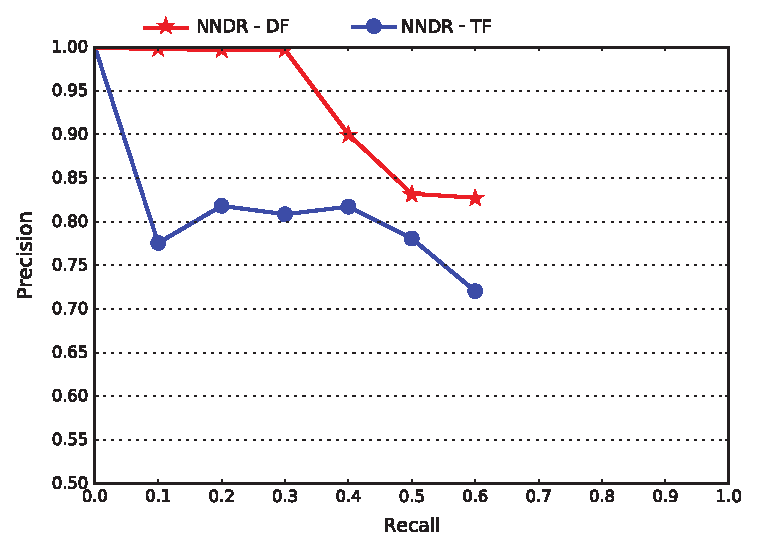
\includegraphics[scale=0.99]{Figures/NNDR_W3G.eps}
\caption{Precision-Recall Curves of NNDR on SANTINIS corpus. The curves are for W3G terms-type and for AUC optimization criterion. The 11-recall-levels are shown for each evaluation experiment. The lines are stopping before the 11th recall level due to the open-set framework, i.e. the remaining part after the last mark of each curve it the percentage of the corpus tha has been classified as Unknown from the algorithms.}
\label{chap:word_embeddings:fig:NNDR_W3G}
\end{center}

\end{figure}

The NNDR-DF is starting higher than NNDR-TF and it remains to $0.99$ precision for the $30\%$ of the corpus. Then it drops rgradualy and remains over $0.80$ up to $60\%$ of the corpus. The the rest of the corpus is classified as unknown. RFSE manages to recognize correctly part of the corpus up to $80\%$ with the precision to drop to $0.70$ and then to $0.65$. 

Considering the NNDR-TF is significantly lower in performance and for the first $10\%$ of the corpus is just above $0.75$. Given that the curves are calculated based on the ranked scores from the best performance to the lowest performance it seems that the algorithm significantly affected by the \textit{unstructured noise}. That is, the algorithm makes very confident decision for some part of the corpus confusing them with other classes. Its overall performance is over $0.7$ precision and also recognize the $60\%$ of the corpus, just like with the DF.

To conclude it seems that NNDR with distributional features is returning a significantly better performance than the BOW with TF weighting scheme. Although the $ΜR$ for PVBOW is slightly lower comparing the last row of both tables \ref{chap:word_embeddings:tbl:NNDR_TF} and \ref{chap:word_embeddings:tbl:NNDR_PVBOW}, the $MP$ is significantly higher. This is more important especially for the task o WGI in an open-set framework with noise, as explained in detail previously (see section \ref{}) in this thesis. 

In the next section the NNDR is compared to the RFSE and OCSVME open-set algorithms both described in \textit{chapter \ref{chap:openset}} and their evaluation experiments presented in \textit{chapter \ref{chap:noise}}.


\subsection{Nearest Neighbours Distance Ration with Paragraph-Vectors}\label{chap:word_embeddings:sec:experiments_setup}

In this section the objective is to find out  how far the improvement of an open-set algorithm can go with the PVBOW neural language model compare to the RFSE and OCSVME as baselines. The baselines and NNDR are applied in the SANTINIS corpus. 

In the training phase, only the 11 known genre classes are use, while in test phase an additional class of the \textit{unstructured noise} is considered. Table\ref{chap:word_embeddings:tbl:NNDR_RFSE_OCSVME_final} shows the performance of tested methods when either TF or DF representation schemes, based on C4G, W1G, or W4G features, are used. 

\begin{table}[t]
\center
\caption {Performance of baselines and NNDR on the SANTINIS coprus. All evaluation scores are macro-averaged.}
\label{chap:word_embeddings:tbl:NNDR_RFSE_OCSVME_final}
\begin{tabular}{ccccccc}
\hline
Model & Features & Dim. & Precision & Recall & AUC & F1 \\
\hline
RFSE & TF-C4G & 50k & 0.739 & \textbf{0.780} & 0.652 & 0.759 \\
RFSE & TF-W1G & 50k & 0.776 & 0.758 & \textbf{0.657} & \textbf{0.767} \\
RFSE & TF-W3G & 50k & 0.797 & 0.722 & 0.615 & 0.758 \\
OCSVM & TF-C4G & 5k & 0.662 & 0.367 & 0.210 & 0.472\\
OCSVM & TF-W1G & 5k & 0.332 & 0.344 & 0.150 & 0.338\\
OCSVM & TF-W3G & 10k & 0.631 & 0.654 & 0.536 & 0.643\\
NNDR & TF-C4G & 5k & 0.664 & 0.403 & 0.291 & 0.502 \\
NNDR & TF-W1G & 5k & 0.691 & 0.439 & 0.348 & 0.537 \\
NNDR & TF-W3G & 10k & 0.720 & 0.664 & 0.486 & 0.691 \\
NNDR & DF-C4G & 50 & \textbf{0.829} & 0.600 & 0.455 & 0.696 \\
NNDR & DF-W1G & 50 & 0.733 & 0.670 & 0.541 & 0.700 \\
NNDR & DF-W3G & 100 & 0.827 & 0.615 & 0.564 & \textbf{0.706} \\
\hline
\end{tabular}
\end{table}

First, NNDR is compared with the baselines using TF features. In this case, NNDR outperforms OCSVM. On the other hand, RFSE performed better than NNDR for MF1 and MAUC. This is consistent for any kind of features (C4G, W1G, or W3G). There is notable difference in the dimensionality of representation used by the examined approaches though. RFSE relies upon a 50k-D manifold while NNDR and OCSVM are based on much lower dimensional spaces. 

The RFSE is the top performer while both OCSVME and NNDR are significantly low in respect of MAUC, MF1 and also MP.  Only, NNDR with TF scheme for W3G is competitive.

Next, NNDR with DF is compared with the same baselines and it self with BOW TF features. As shown in section \ref{chap:word_embeddings:sec:NNDR_PVBOW_vs_BOW} above there is a notable improvement for NNDR with DF features and now is comparable with RFSE baseline. 

However, still RFSE outperforms NNDR although the MF1 is comparable for all cases of features, i.e. W3G, W1G, C4G. On the other hand NNDR returns an notably higher performance from RFSE in respect of MP for C4G and W3G. It also to be noted that in all cases the selected value of parameter DRT is 0.8. This indicates that NNDR is a very robust algorithm.

The dimensionality of DF is much lower than TF and this seems to be crucial to improve the performance of NNDR. This is consistent for all three feature types (C4G, W1G, and W3G). It has to be noted that RFSE builds an ensemble by iteratively and \textit{randomly selecting} a subset of the available features. That way, it internally reduces the dimensionality for each constituent base classifier. RFSE is using about 1000 \textit{randomly selected features} from the 50,000 most frequent features. This observations together with the improvement of the NNDR performance with DF is a strong indication where the genre information is pervasive in several features of the texts and the magnitude of the features frequency is not enough. 

Finally, the proposed approach using NNDR and DF outperforms OCSVM but, as said above, it is outperformed by the strong baseline RFSE in both MAUC and MF1. However, when precision is concerned, NNDR is much better. A closer look at  the comparison of the two methods is provided in Fig. \ref{chap:word_embeddings:fig:NNDR_W3G_Best_RFSE_Baseline}, where MPRCs are depicted. 

The NNDR-DF model maintains very high precision scores for low levels of recall. Particularly, for W3G the difference between NNDR-DF and RFSE at that point is clearer. NNDR-TF is clearly worse than both NNDR-DF and RFSE. In addition, OCSVM is competitive in terms of precision only when W3G features are used but its performance drops abruptly in comparison to that of NNDR-DF. 

RFSE with W1G performs significantly better in terms of MP than NNDR (with DF). It also manages to recognize correctly larger part of the corpus, more than $70\%$ either for W3G or for W1G, compare to NNDR-DF that reaches $60\%$ in both left and right diagrams of figure \ref{chap:word_embeddings:fig:NNDR_W3G_Best_RFSE_Baseline}. Note that the point where the curves end indicates the percentage of corpus that is left unclassified because it is left unclassified as \tetxit{unknown class}.

\begin{figure}[t]
\begin{center}
    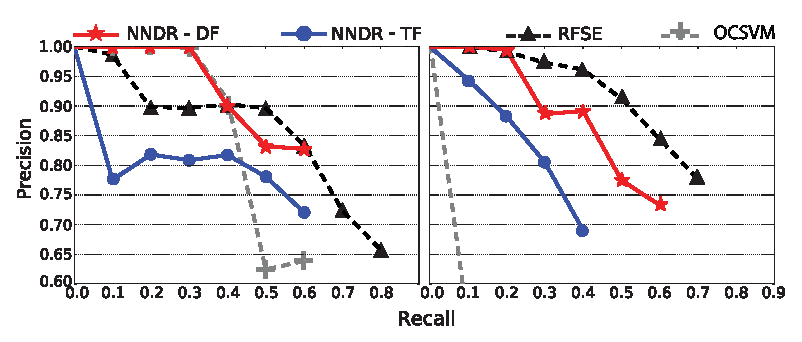
\includegraphics[scale=0.95]{Figures/NNDR_W3G-W1G_Best_RFSE-OCSVM-Baselines.eps}
	\caption{Precision curves in 11-standard recall levels of the examined open-set classifiers using either W3G features (left) or W1G features (right).}
	\label{chap:word_embeddings:fig:NNDR_W3G_Best_RFSE_Baseline}
	\end{center}
\end{figure}

%, i.e. the remaining part after the last mark of each curve it the percentage of the corpus tha has been classified as Unknown from the algorithms.

\section{Conclusions}\label{chap:word_embeddings:sec:conclusions}

In this chapter is presented an experimental study focused on WGI and the use of distributional features in combination with an open-set classifier that obtained promising results in other domains. Our experiments are based on a benchmark corpus already used in prior art and a strong baseline. Particularly it is evaluated the possible performance improvement of an open-set algorithm when distributional features are employed, using the SANTINIS corpus (i.e. a corpus with an unstructured noise).

It seems that distributional features provide a significant enhancement to the NNDR open-set method. The low-dimensionality of DF is crucial to boost the performance of NNDR. Yet, RFSE proves to be a hard-to-beat baseline at the expense of relying upon a much higher representation space (usually in the thousands of features). However, with respect to precision, the NNDR with PVBOW neural model input, is much more conservative and it prefers to leave web-pages unclassified rather than guessing an inaccurate genre label. Depending on the application of WGI, precision can be considered much more important than recall and this is where the proposed approach shines, i.e an open-set algorithm combined with \tetxit{neural language model}.

The open-set algorithm NNDR have been evaluated with distributional features which have been described in detail in chapter \ref{chap:openset}. A \textDistance Ration threshold is calculated while the training procedure for maximizing the \textit{Normalized Accuracy} of the known and the unknown classes.

The evaluation methodology previews shown to be proper for evaluation open-set scenarios. The natural focus in an open-set evaluation framework is the macro-precision, because always there is a part of the corpus will be classified as unknown. Either in the case of structured and unstructured or it is considered as outage while training.

Further research could focus on more appropriate distance measures within NNDR specially with recent data-driven features obtained with powerful NLP convolutional and recurrent deep networks. Moreover, alternative types of distributional features could be used (e.g., topic modeling). Finally, a combination of NNDR with RFSE models could be studied as they seem to exploit complementary views of the same problem.

